\documentclass{article}

\usepackage[margin=1in]{geometry}
\usepackage[center]{caption}
\usepackage{subfigure}
\usepackage{appendix}
\usepackage{amsmath}
\usepackage{graphicx}
\usepackage{todonotes}
\usepackage{tikz}

\usetikzlibrary{fit,positioning}

\newcommand{\HRule}{\rule{\linewidth}{0.1mm}}

\begin{document}

\title{ \HRule \\[0.2cm]
		Autonomous Agents\\ 
		Report Assignment 2: Single Agent Learning\\
		\HRule \\[0.1cm]
		}
		
\author{
		\emph{Authors:}\\[0.2cm]
		Agnes \textsc{van Belle} \small{ \emph{(10363130)}},\\ 
		Maaike \textsc{Fleuren} \small{ \emph{(10350470)}}, \\
		Norbert \textsc{Heijne} \small{ \emph{(10357769)}}, \\
		Lydia \textsc{Mennes} \small{ \emph{(10333843)}}
		}
		
\maketitle

\section{Introduction}
This report has been written for the Master Artificial Intelligence course Autonomous Agents. This report will contain the answers, motivation and explanation for our implementations of the tasks we had to accomplish in our second assignment for this course. These tasks were centered around the topic of `Single Agent Learning'.

\subsection{The environment} \label{sec:environment}
In all tasks there is assumed to be a grid world (of $11 \times 11$) with a predator and a prey in it. The agents can both move one tile forward each iteration. The direction they take (or if they move at all) is affected by probabilities (their policies). If they move over the edge of the grid they end up at the opposing side of the grid. The prey will never step onto the predator. We are focused on improving the decisions of one agent, the predator. 

\subsection{The state space representation} \label{sec:stateSpace}
In the experiments described the first report, we initially used a state space that was an intuitive, yet cumbersome representation. We referred to that state space representation as the `default' state space. The amount of states that was used in the default state space was $(11 \times 11) \times (11 \times 11) = 121 \times 121 = 14641$. We then changed the state space representation to a more efficient one, referred to as the `efficient' state space, which led to a reduction of 697 times less states, resulting in just 21 different states.

In this assignment, we used this efficient state space representation for the learning algorithms. To give a good understanding of our learning algorithms, which were built on the efficient state space representation, we will once again explain how this representation works.

Figure \ref{fig:statespaceSymm} illustrates that there is a symmetry in the default state space, and thus that there were relatively much values redundantly computed.
By using this symmetry in the default state space a much smaller state space was achieved. 

Each state represents a distance between the prey and predator. These are represented in the lower left diagonal of a matrix, in which the $x$-axis is the relative horizontal distance in the MDP and the $y$-axis the relative vertical distance in the MDP. This matrix is shown in Figure \ref{fig:NewStateRep}. Combinations of positions of prey and predator for which the horizontal and vertical distances are equal are now treated equivalent. 
Also two combinations for which the horizontal distance in one equals the vertical distance in the other and vice versa are considered equal. In order to navigate through this state space different actions are required. These are: \textit{horizontal retreat, horizontal approach, vertical retreat, vertical approach}, as illustrated in Figure \ref{fig:statespaceSymm}, and of course the action \textit{wait}. When interacting with the environment these actions are converted into corresponding actions in the real world. This only requires the relative direction of the prey (which is always located at the centre, regardless of its coordinates) with respect to the predator. This is computed by using the difference in location of the prey and predator on the $x$- and $y$-axis.

\begin{figure}[ht]
\centering
\subfigure[The $11 \times 11$ grid divided into eight symmetric pieces, with the corresponding possible moves which are also symmetric.]{
    \includegraphics[width=0.5\textwidth]{statespaceSymm.png}
    \label{fig:statespaceSymm}
}
\subfigure[Colormap of $V$-values, the brighter the color the higher the corresponding $V$-value. The prey is always located on the (1, 1) coordinate in this state representation.]{
    \includegraphics[width=0.4\textwidth]{VMatrixNewStateRep.png}
    \label{fig:NewStateRep}
}
\caption{Illustration of the symmetry and corresponding values of the new state space representation}
\label{fig:statespaceIll}
\end{figure}


\subsection{Implementation details}
This report will not be about our exact code and implementation details. However, a class diagram of our code is provided in Appendix \ref{app:classDiagram}.

\section{Learning algorithms}
As mentioned before, we will use the same environment as in the previous assignment. But in this assignment, we will assume the learning scenerio: the agent does not know the transition probabilities, nor the reward structure. On a very high level there are two ways to come to a good solution in this setting: learning the model, and do planning again (model based learning), or not learn the model, and directly try to learn a high-reward policy (model-free learning). In this assignment we will focus on the latter.\footnote{Roijers (2012) \textit{Assignments Autonomous Agents} p. 6}

\subsection{(M) Q-Learning}\label{sec:exercise1}
Q-Learning is an off-policy temporal-difference control algorithm. Temporal-difference methods can learn directly from raw experience without a model of the environment's dynamics. Furthermore, it updates estimates based in part on other learned estimates, without waiting for a final outcome.\footnote{Sutton, Barto (1998) \textit{Reinforcement Learning: An Introduction} Cambridge, Massachusetts: The MIT press. p. 133}

While the distinguishing feature of on-policy methods is that they estimate the value of a policy while using it for control, these two functions are separated in off-policy methods. The behavior policy, used to generate behavior, and the estimation policy, that is evaluated and improved, may in fact be unrelated. This separation is an advantage because the estimation policy may be deterministic (e.g., greedy), while the behavior policy can continue to sample all possible actions.\footnote{Sutton, Barto (1998) \textit{Reinforcement Learning: An Introduction} Cambridge, Massachusetts: The MIT press. p. 126} Its simplest form, \textit{one-step Q-learning}, is defined by\footnote{Sutton, Barto (1998) \textit{Reinforcement Learning: An Introduction} Cambridge, Massachusetts: The MIT press. p. 148}:
\begin{align*}
Q(s_t,a_t) & \leftarrow Q(s_t,a_t) + \alpha \left[ r_{t+1} + \gamma \displaystyle\max_a Q(s_{t+1},a) - Q(s_t,a_t) \right]
\end{align*}

For this assignment, we implemented Q-learning and used it for our predator agent. We used $\epsilon$-greedy action selection, which behaves greedily most of the time, but with probability $\epsilon$, instead select an action at random, uniformly, independently of the action-value estimates.\footnote{Sutton, Barto (1998) \textit{Reinforcement Learning: An Introduction} Cambridge, Massachusetts: The MIT press. p. 28} In this case, we used $\epsilon = 0.1$. We initiated the values of our Q-learning table optimistically with a value of 15 for all cells in the table.

Figure \ref{plot:QLearningAlpha} shows plots on the performance of the agent over time for different $\alpha$ (learning rate) and figure  \ref{plot:QLearningGamma} for different $\gamma$ (discount factor) using $\epsilon$-greedy action selection.

A few observations can be made on these results. The values of $\alpha$ higher than 0.5 seem to have an adverse effect on the agent's performance for both the NRMSE (Normalized-Root-Mean-Squared-Error) and the percentage of optimal actions measures. As the $\alpha$ increases from 0.1 to 0.5, the performance increases over first 100 episodes for both measures, which is not the case for $\alpha$=0.7 as seen in figure \ref{plot:QLearningAlpha}. 

The values of 0.1, 0.5 and 0.7 for $\gamma$ seem to have an early advantage over the value 0.9 for $\gamma$ in beginning of the runs as seen in figure \ref{plot:QLearningGamma}. This can be explained by the fact that a lower $\gamma$ makes the state action pair values fluctuate much faster than a higher $\gamma$, so that early on the values might be better, but as the number of episodes increases, the values of the state action pairs drops further which in turn increases the NRMSE. However, looking at the percentage of optimal actions, the performance is on par with $\gamma$=0.9. Which means that even though the values might be low, the resulting policy would perform just as well.

\begin{figure}[ht]
\centering
\subfigure[A comparison of the performance of the agent based on the resulting Normalized-Root-Mean-Squared-Error of the agent's state action pairs and the the estimated true state action pairs.]{
    \includegraphics[width=0.45\textwidth]{QLearningAlphaNRMSE.png}
    \label{fig:QLearningAlphaNRMSE}
}
\subfigure[A comparison of the performance of the agent based on the resulting percentage of best actions in the state space action pairs $\displaystyle\max_a Q(s_t,a_t)$ of the agent that are also present as the best actions in the estimated true state action pairs.]{
    \includegraphics[width=0.45\textwidth]{QLearningAlphaOA.png}
    \label{fig:QLearningAlphaOA}
}
\caption{Plots on the performance of the agent over time for different values of the learning rate $\alpha$ using $\epsilon$-greedy action selection. Averaged over 100 runs with 1000 episodes each with $\epsilon = $ 0.1 and the discount factor $\gamma$ = 0.9.}
\label{plot:QLearningAlpha}
\end{figure}

\begin{figure}[ht]
\centering
\subfigure[A comparison of the performance of the agent based on the resulting Normalized-Root-Mean-Squared-Error of the agent's state action pairs and the the estimated true state action pairs.]{
    \includegraphics[width=0.45\textwidth]{QLearningGammaNRMSE.png}
    \label{fig:QLearningGammaNRMSE}
}
\subfigure[A closeup of the first 100 episodes of figure \ref{fig:QLearningGammaNRMSE}.]{
    \includegraphics[width=0.45\textwidth]{QLearningGammaNRMSE_detail.png}
    \label{fig:QLearningGammaNRMSE_detail}
}
\subfigure[A comparison of the performance of the agent based on the resulting percentage of best actions in the state space action pairs of the agent that are also present as the best actions in the estimated true state action pairs.]{
    \includegraphics[width=0.45\textwidth]{QLearningGammaOA.png}
    \label{fig:QLearningGammaOA}
}
\caption{Plots on the performance of the agent over time for different values of the discount factor $\gamma$ using $\epsilon$-greedy action selection. Averaged over 100 runs with 1000 episodes each with $\epsilon = $ 0.1 and the learning rate $\alpha$ = 0.5.}
\label{plot:QLearningGamma}
\end{figure}

\subsection{(M) Experiment with $\epsilon$ and optimistic initialization}\label{sec:exercise2}

The values chosen to evaluate were the combinations of a low initialization value (neutral initialization), a high initialization value (optimistic initialization), a low value for $\epsilon$ (close to greedy policy) and a high value for $\epsilon$ (exploratory/random policy). From these results we can make a few observations. 

\begin{figure}[ht]
\centering
\subfigure[A comparison of the performance of the agent based on the average number of steps taken for each episode.]{
    \includegraphics[width=0.45\textwidth]{secondMust_nrSteps.png}
    \label{fig:secondMust_nrSteps}
}
\subfigure[A comparison of the performance of the agent based on the resulting percentage of best actions in the state space action pairs of the agent that are also present as the best actions in the estimated true state action pairs.]{
    \includegraphics[width=0.45\textwidth]{secondMust_optimalAction.png}
    \label{fig:secondMust_optimalAction}
}
\subfigure[A closeup of the first 20 episodes of figure \ref{fig:secondMust_nrSteps}.]{
    \includegraphics[width=0.45\textwidth]{secondMust_nrSteps_detail.png}
    \label{fig:secondMust_nrSteps_detail}
}
\subfigure[A comparison of the performance of the agent based on the percentage of state action pairs visited after each episode.]{
    \includegraphics[width=0.45\textwidth]{secondMust_visitedPairs_detail.png}
    \label{fig:secondMust_visitedPairs_detail}
}
\caption{Plots on the performance of the agent over time for different values of $\epsilon$ and initialization values using $\epsilon$-greedy action selection. Averaged over 100 runs with 1000 episodes each with $\gamma = $ 0.9 and the learning rate $\alpha$ = 0.5.}
\label{plot:secondMust}
\end{figure}

\subsection{(SC) Softmax action selection instead of $\epsilon$-greedy}\label{sec:exercise3}
For this exercise we will try to illustrate the difference between $\epsilon$-greedy and softmax. These two methods are both for action selection and this will most likely have an impact on the way that the state action pairs are explored. $\epsilon$-greedy will have a fixed chance of trying to explore a random action for the current state. For softmax the greedy action is still given the highest selection probability, but all the others are ranked and weighted according to their value estimates.\footnote{Suttion, Barto (1998) \textit{Reinforcement Learning: An Introduction} Cambridge, Massachusetts: The MIT press. p. 30} 

Through the following plots in figure \ref{plot:secondShould} we will show the effects of the different values of $\tau$ and $\epsilon$ on exploration. The performance of both algorithms seem to be on par with each other, and show very similar behavior. 

Figure \ref{plot:QSalphagamma} shows plots on the performance of the agent over time for different $\alpha$ and for different $\gamma$ (discount factor), this time using softmax action selection.

\begin{figure}[ht]
\centering
\subfigure[A comparison of the performance of the agent based on the average number of steps taken for each episode.]{
    \includegraphics[width=0.45\textwidth]{secondShould_Greedy_nrSteps.png}
    \label{fig:secondShould_Greedy_nrSteps}
}
\subfigure[A comparison of the performance of the agent based on the average number of steps taken for each episode.]{
    \includegraphics[width=0.45\textwidth]{secondShould_Softmax_nrSteps.png}
    \label{fig:secondShould_Softmax_nrSteps}
}
\subfigure[A comparison of the performance of the agent based on the resulting percentage of best actions in the state space action pairs of the agent that are also present as the best actions in the estimated true state action pairs.]{
    \includegraphics[width=0.45\textwidth]{secondShould_Greedy_OA.png}
    \label{fig:secondShould_Greedy_OA}
}
\subfigure[A comparison of the performance of the agent based on the resulting percentage of best actions in the state space action pairs of the agent that are also present as the best actions in the estimated true state action pairs.]{
    \includegraphics[width=0.45\textwidth]{secondShould_Softmax_OA.png}
    \label{fig:secondShould_Softmax_OA}
}
\subfigure[A comparison of the performance of the agent based on the percentage of state action pairs visited after each episode.]{
    \includegraphics[width=0.45\textwidth]{secondShould_Greedy_visitedPairs.png}
    \label{fig:secondShould_Greedy_visitedPairs}
}
\subfigure[A comparison of the performance of the agent based on the percentage of state action pairs visited after each episode.]{
    \includegraphics[width=0.45\textwidth]{secondShould_Softmax_visitedPairs.png}
    \label{fig:secondShould_Softmax_visitedPairs}
}
\caption{Plots on the performance of the agent over time for different values of $\epsilon$ using $\epsilon$-greedy action selection (figures \ref{fig:secondShould_Greedy_nrSteps}, \ref{fig:secondShould_Greedy_OA} and \ref{fig:secondShould_Greedy_visitedPairs}) and for different values of $\tau$ using the Softmax action selection (figures \ref{fig:secondShould_Softmax_nrSteps}, \ref{fig:secondShould_Softmax_OA} and \ref{fig:secondShould_Softmax_visitedPairs}). Averaged over 100 runs with 1000 episodes each with $\gamma = $ 0.9, the learning rate $\alpha$ = 0.5 and the initialization value at 15.}
\label{plot:secondShould}
\end{figure}

\todo[inline, color=yellow]{Experiment with different values of $\epsilon$ and the optimistic initialization of the Q-table. Make up good values to test, and explain why you chose these values.}

\subsection{(SC) Softmax action selection instead of $\epsilon$-greedy}\label{sec:exercise3}
For this exercise, we did the same as we did in section \ref{sec:exercise1}, but instead of using $\epsilon$-greedy action selection we used softmax action selection. This means that the greedy action is still given the highest selection probability, but all the others are ranked and weighted according to their value estimates.\footnote{Sutton, Barto (1998) \textit{Reinforcement Learning: An Introduction} Cambridge, Massachusetts: The MIT press. p. 30}

Figure \ref{plot:QSalphagamma} shows plots on the performance of the agent over time for different $\alpha$ and for different $\gamma$ (discount factor), this time using softmax action selection.

%\begin{figure}
\missingfigure{Plots on the performance of the agent over time for different $\alpha$ and for different $\gamma$ (discount factor) using softmax action selection.} \label{plot:QSalphagamma}
%\end{figure}

\todo[inline, color=yellow]{Illustrate the difference between $\epsilon$-greedy and softmax, using graphs from your empirical results.}

\subsection{Other ways to do learning}

\subsubsection{(SC) On-policy Monte Carlo Control}\label{sec:exercise4.1}
As mentioned in section \ref{sec:exercise1}, on-policy methods try to evaluate or improve the policy that is used to make decisions.\footnote{Sutton, Barto (1998) \textit{Reinforcement Learning: An Introduction} Cambridge, Massachusetts: The MIT press. p. 122} Monte Carlo estimation can be used to approximate optimal policies, which results in Monte Carlo control. It proceeds according to the idea of generalized policy iteration, where one maintains both an approximate policy and an approximate value function. The value function is repeatedly altered to more closely approximate the value function for the current policy, and the policy is repeatedly improved with respect to the current value function.\footnote{Sutton, Barto (1998) \textit{Reinforcement Learning: An Introduction} Cambridge, Massachusetts: The MIT press. p. 118} In this case, our policy moves towards a softmax policy, which was previously explained in section \ref{sec:exercise3}. Furthermore, it is necessary to use either exploring starts or and $\epsilon$-soft policy because making the policy greedy prevents further exploration of nongreedy actions. Since an assumption of exploring starts is an unlikely assumption an $\epsilon$-soft policy is used in this case: softmax.\\ 

On Policy Monte Carlo Control differs from other methods in the fact that the agent does not learn until the end of an episode. Such an episode can be regarded as a sample which is then used to update the Q-values of the encountered state-action pairs. Learned information can therefore not be used until the next episode.\\ 

There are a number of parameters used in the implementation of this learning method. The first parameter is $\tau$ for the softmax policy, determining how much the agent will explore. The number of runs which determines how much the agent will learn. The initialization for the Q-values which is still optimistic and the discount factor $\lambda$.\\  

How the number of steps needed to catch a prey changes over the number of runs for different parameter settings can be seen in figures \ref{fig:onLineMonteCarloDiscount} and \ref{fig:onLineMonteCarloTau}. The resulting policy can be found in Appendix \ref{policyOnLineMonteCarlo}.

\begin{figure}
\centering
\caption{Number of steps for each episode as the agent learns for different values of the discount factor. The values are averaged over 50 trials where the agent learns for 100 runs. The value of $\tau$ is set to 0.9}
\label{fig:onLineMonteCarloDiscount}
\includegraphics[scale=0.8]{averagesInOneFig_online_discountFact.png}
\end{figure}

\begin{figure}
\centering
\caption{Number of steps for each episode as the agent learns for different values of $\tau$. The values are averaged over 50 trials where the agent learns for 100 runs. The value of the discount factor is set to 0.8}
\label{fig:onLineMonteCarloTau}
\includegraphics[scale=0.8]{averagesInOneFig_online_Tau.png}
\end{figure}


\todo[inline, color=yellow]{Explain the difference with other learning methods theoretically, and compare them using informative graphs.}

\subsubsection{(SC) Off-Policy Monte Carlo Control}\label{sec:exercise4.2}

Off-policy Monte Carlo control follows the behavior policy while learning about and improving the estimation policy, which makes it different from other learning methods.\footnote{Sutton, Barto (1998) \textit{Reinforcement Learning: An Introduction} Cambridge, Massachusetts: The MIT press. p. 126} The behavior policy is a $\epsilon$-soft policy and therefore keeps exploring, while the estimation policy can be a deterministic greedy policy. In order to transfer the learned information from the behavior policy to the estimation policy importance sampling is used, since the probability of taking an action in one policy is not the same as in the other.\\

In this specific case the behavior policy is a softmax policy learned with the on-line Monte Carlo method, using 600 runs, a discount factor of 0.9 and $\tau$ is set to 0.9.

How the number of steps per episodes changes dusring learning in this implementation can be seen in figure \ref{offLine}. The resulting policy can be found in Appendix \ref{policyOffLineMonteCarlo}.

\begin{figure}
\centering
\label{offLine}
\caption{The number of steps for each episode averaged over 5 trials where the agent learns for 150 runs}
\includegraphics[scale=0.8]{offpolicy.png}
\end{figure}



\subsubsection{(SC) Sarsa}\label{sec:exercise4.3}
\textit{For an explanation of on-policy methods and temporal difference learning, please take a look at section \ref{sec:exercise1} or \ref{sec:exercise4.1}, and section \ref{sec:exercise1} respectively.}
\\ \\
In contrast to the Q-learning method, Sarsa is an on-policy temporal-difference control algorithm. Just like Q-learning it learns an action-value function rather than a state-value function, but for an on-policy method like Sarsa we must estimate $Q^\pi (s,a)$ for the current behavior policy $\pi$ and for all states $s$ and actions $a$.\footnote{Sutton, Barto (1998) \textit{Reinforcement Learning: An Introduction} Cambridge, Massachusetts: The MIT press. p. 145}

In Sarsa we consider transitions from state-action pair to state-action pair, and learn the value of state-action pairs. An alternating sequence of of states and state-action pairs forms an episode:

\begin{center}
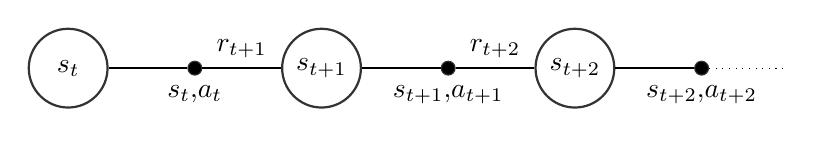
\begin{tikzpicture}
\tikzstyle{main}=[circle, minimum size = 10mm, thick, draw =black!80, node distance = 10mm]
\tikzstyle{connect}=[-, thick]
\tikzstyle{dot}=[circle, inner sep=0pt,minimum size=5pt, draw =black!80, fill=black, node distance = 10mm]
\tikzstyle{empty}=[rectangle, fill=white, node distance=10mm]
  \node[main, fill = white!100] (st) [] {$s_t$};
\node[dot] (stat) [right=of st, label=below:$s_t \text{,} a_t$] {};
  \node[main] (st1) [right=of stat] {$s_{t+1}$};
\node[dot] (st1at1) [right=of st1, label=below:$s_{t+1}\text{,} a_{t+1}$] {};
\node[main] (st2) [right=of st1at1] {$s_{t+2}$};
\node[dot] (st2at2) [right=of st2, label=below:$s_{t+2}\text{,} a_{t+2}$] {}; 
\node[empty] (empty) [right=of st2at2] {};

  \path (st) edge [connect] (stat)
        (stat) edge [connect] node[auto] {$r_{t+1}$} (st1)
	(st1) edge [connect] (st1at1)
	(st1at1) edge [connect] node[auto] {$r_{t+2}$} (st2)
	(st2) edge [connect] (st2at2);
\draw [dotted] (st2at2) -- (empty);
  \end{tikzpicture}
\end{center}

After every transition from a nonterminal state $s_t$ an update is done:

\begin{align*}
Q(s_t,a_t) & \leftarrow Q(s_t,a_t) + \alpha \left[ r_{t+1} + \gamma \, Q(s_{t+1},a_{t+1}) - Q(s_t,a_t) \right]
\end{align*}
If $s_{t+1}$ is terminal, then $Q(s_{t+1},a_{t+1})$ is defined as zero. As you can see, this update uses every element that makes up a transition from one state-action pair to the next ($s_t,a_t,r_{t+1},s_{t+1},a_{t+1}$), from which the name Sarsa originates.

\todo[inline, color=yellow]{Explain the difference with other learning methods theoretically, and compare them using informative graphs.}

\section{Conclusion}

\newpage
\nocite{*}
\bibliographystyle{plainnat}
\bibliography{references}

\newpage
\appendix
\appendixpage
<<<<<<< HEAD
\section{Class Diagram} \label{app:classDiagram}
\appendixpage
\section{Policy of On Line Monte Carlo} \label{policyOnLineMonteCarlo}
The policy resulting from On Line Monte Carlo learning can be found in Table \ref{policyOnline}
 \begin{table}[htbp]
\caption{The policy resulting from On Line Monte Carlo learning method with $\tau$ is 0.9 and discount factor is 0.9 after 500 episodes}
\label{policyOnline}
\centering
\begin{footnotesize}
\begin{tabular}{c|c|c|c|c|c|c|c|c|c|c|c|}
&0&1&2&3&4&5&6&7&8&9&10\\ \hline\\
0&U 0,189&U 0,176&U 0,181&U 0,149&U 0,120&U 0,097&U 0,120&U 0,149&U 0,181&U 0,176&U 0,189\\
&R 0,220&R 0,239&R 0,250&R 0,241&R 0,132&R 0,078&R 0,118&R 0,119&R 0,132&R 0,165&R 0,194\\
&D 0,207&D 0,234&D 0,263&D 0,317&D 0,421&D 0,575&D 0,421&D 0,317&D 0,263&D 0,234&D 0,207\\
&L 0,194&L 0,165&L 0,132&L 0,119&L 0,118&L 0,046&L 0,132&L 0,241&L 0,250&L 0,239&L 0,220\\
&W 0,190&W 0,186&W 0,173&W 0,175&W 0,209&W 0,203&W 0,209&W 0,175&W 0,173&W 0,186&W 0,190\\
\hline \\
1&U 0,165&U 0,137&U 0,118&U 0,070&U 0,050&U 0,036&U 0,050&U 0,070&U 0,118&U 0,137&U 0,176\\
&R 0,234&R 0,276&R 0,335&R 0,359&R 0,357&R 0,046&R 0,040&R 0,069&R 0,107&R 0,135&R 0,165\\
&D 0,239&D 0,282&D 0,250&D 0,349&D 0,424&D 0,752&D 0,424&D 0,349&D 0,250&D 0,282&D 0,234\\
&L 0,176&L 0,135&L 0,107&L 0,069&L 0,040&L 0,129&L 0,357&L 0,359&L 0,335&L 0,276&L 0,239\\
&W 0,186&W 0,169&W 0,190&W 0,152&W 0,128&W 0,037&W 0,128&W 0,152&W 0,190&W 0,169&W 0,186\\
\hline \\
2&U 0,132&U 0,107&U 0,083&U 0,056&U 0,004&U 0,003&U 0,004&U 0,056&U 0,083&U 0,118&U 0,132\\
&R 0,263&R 0,250&R 0,299&R 0,403&R 0,301&R 0,003&R 0,054&R 0,048&R 0,074&R 0,107&R 0,181\\
&D 0,250&D 0,335&D 0,433&D 0,344&D 0,550&D 0,944&D 0,550&D 0,344&D 0,433&D 0,250&D 0,250\\
&L 0,181&L 0,118&L 0,074&L 0,048&L 0,054&L 0,048&L 0,301&L 0,403&L 0,299&L 0,335&L 0,263\\
&W 0,173&W 0,190&W 0,111&W 0,150&W 0,090&W 0,003&W 0,090&W 0,150&W 0,111&W 0,190&W 0,173\\
\hline \\
3&U 0,119&U 0,069&U 0,048&U 0,012&U 0,031&U 0,053&U 0,031&U 0,012&U 0,056&U 0,069&U 0,119\\
&R 0,317&R 0,349&R 0,344&R 0,672&R 0,092&R 0,001&R 0,052&R 0,007&R 0,048&R 0,070&R 0,149\\
&D 0,241&D 0,359&D 0,403&D 0,110&D 0,822&D 0,941&D 0,822&D 0,110&D 0,344&D 0,359&D 0,241\\
&L 0,149&L 0,070&L 0,056&L 0,007&L 0,052&L 0,001&L 0,092&L 0,672&L 0,403&L 0,349&L 0,317\\
&W 0,175&W 0,152&W 0,150&W 0,199&W 0,002&W 0,004&W 0,002&W 0,199&W 0,150&W 0,152&W 0,175\\
\hline \\
4&U 0,118&U 0,040&U 0,054&U 0,052&U 0,019&U 0,001&U 0,019&U 0,031&U 0,054&U 0,040&U 0,118\\
&R 0,421&R 0,424&R 0,550&R 0,822&R 0,977&R 0,144&R 0,003&R 0,052&R 0,004&R 0,050&R 0,120\\
&D 0,132&D 0,357&D 0,301&D 0,092&D 0,001&D 0,855&D 0,001&D 0,822&D 0,301&D 0,357&D 0,132\\
&L 0,120&L 0,050&L 0,004&L 0,031&L 0,003&L 0,000&L 0,977&L 0,092&L 0,550&L 0,424&L 0,421\\
&W 0,209&W 0,128&W 0,090&W 0,002&W 0,001&W 0,000&W 0,001&W 0,002&W 0,090&W 0,128&W 0,209\\
\hline \\
5&U 0,046&U 0,129&U 0,048&U 0,001&U 0,000&&U 0,001&U 0,001&U 0,048&U 0,129&U 0,046\\
&R 0,575&R 0,752&R 0,944&R 0,941&R 0,855&&R 0,000&R 0,053&R 0,003&R 0,036&R 0,097\\
&D 0,078&D 0,046&D 0,003&D 0,001&D 0,144&Prey&D 0,855&D 0,001&D 0,003&D 0,046&D 0,078\\
&L 0,097&L 0,036&L 0,003&L 0,053&L 0,001&&L 0,144&L 0,941&L 0,944&L 0,752&L 0,575\\
&W 0,203&W 0,037&W 0,003&W 0,004&W 0,000&&W 0,000&W 0,004&W 0,003&W 0,037&W 0,203\\
\hline \\
6&U 0,132&U 0,357&U 0,301&U 0,092&U 0,977&U 0,855&U 0,977&U 0,092&U 0,301&U 0,357&U 0,132\\
&R 0,421&R 0,424&R 0,550&R 0,822&R 0,001&R 0,144&R 0,019&R 0,031&R 0,004&R 0,050&R 0,120\\
&D 0,118&D 0,040&D 0,054&D 0,052&D 0,003&D 0,001&D 0,003&D 0,052&D 0,054&D 0,040&D 0,118\\
&L 0,120&L 0,050&L 0,004&L 0,031&L 0,019&L 0,000&L 0,001&L 0,822&L 0,550&L 0,424&L 0,421\\
&W 0,209&W 0,128&W 0,090&W 0,002&W 0,001&W 0,000&W 0,001&W 0,002&W 0,090&W 0,128&W 0,209\\
\hline \\
7&U 0,241&U 0,359&U 0,403&U 0,672&U 0,822&U 0,941&U 0,822&U 0,672&U 0,403&U 0,359&U 0,241\\
&R 0,317&R 0,349&R 0,344&R 0,110&R 0,092&R 0,001&R 0,052&R 0,012&R 0,056&R 0,070&R 0,149\\
&D 0,119&D 0,069&D 0,048&D 0,007&D 0,031&D 0,053&D 0,031&D 0,007&D 0,048&D 0,069&D 0,119\\
&L 0,149&L 0,070&L 0,056&L 0,012&L 0,052&L 0,001&L 0,092&L 0,110&L 0,344&L 0,349&L 0,317\\
&W 0,175&W 0,152&W 0,150&W 0,199&W 0,002&W 0,004&W 0,002&W 0,199&W 0,150&W 0,152&W 0,175\\
\hline \\
8&U 0,250&U 0,335&U 0,299&U 0,344&U 0,550&U 0,944&U 0,550&U 0,344&U 0,299&U 0,335&U 0,250\\
&R 0,263&R 0,250&R 0,433&R 0,403&R 0,301&R 0,003&R 0,054&R 0,048&R 0,083&R 0,118&R 0,181\\
&D 0,132&D 0,107&D 0,074&D 0,056&D 0,004&D 0,003&D 0,004&D 0,056&D 0,074&D 0,107&D 0,132\\
&L 0,181&L 0,118&L 0,083&L 0,048&L 0,054&L 0,048&L 0,301&L 0,403&L 0,433&L 0,250&L 0,263\\
&W 0,173&W 0,190&W 0,111&W 0,150&W 0,090&W 0,003&W 0,090&W 0,150&W 0,111&W 0,190&W 0,173\\
\hline \\
9&U 0,239&U 0,276&U 0,250&U 0,349&U 0,424&U 0,752&U 0,424&U 0,349&U 0,250&U 0,276&U 0,239\\
&R 0,234&R 0,282&R 0,335&R 0,359&R 0,357&R 0,046&R 0,040&R 0,069&R 0,107&R 0,137&R 0,176\\
&D 0,165&D 0,135&D 0,118&D 0,070&D 0,050&D 0,036&D 0,050&D 0,070&D 0,118&D 0,135&D 0,165\\
&L 0,176&L 0,137&L 0,107&L 0,069&L 0,040&L 0,129&L 0,357&L 0,359&L 0,335&L 0,282&L 0,234\\
&W 0,186&W 0,169&W 0,190&W 0,152&W 0,128&W 0,037&W 0,128&W 0,152&W 0,190&W 0,169&W 0,186\\
\hline \\
10&U 0,220&U 0,234&U 0,263&U 0,317&U 0,421&U 0,575&U 0,421&U 0,317&U 0,263&U 0,234&U 0,220\\
&R 0,207&R 0,239&R 0,250&R 0,241&R 0,132&R 0,078&R 0,118&R 0,119&R 0,132&R 0,165&R 0,189\\
&D 0,194&D 0,176&D 0,181&D 0,149&D 0,120&D 0,097&D 0,120&D 0,149&D 0,181&D 0,176&D 0,194\\
&L 0,189&L 0,165&L 0,132&L 0,119&L 0,118&L 0,046&L 0,132&L 0,241&L 0,250&L 0,239&L 0,207\\
&W 0,190&W 0,186&W 0,173&W 0,175&W 0,209&W 0,203&W 0,209&W 0,175&W 0,173&W 0,186&W 0,190\\
\hline \\
\end{tabular}
\end{footnotesize}
\end{table}
\section{Policy of Off Line Monte Carlo} \label{policyOffLineMonteCarlo}
The policy resulting from Off Line Monte Carlo learning can be found in Table \ref{policyOffline}
 \begin{table}[htbp]
\caption{The estimation policy resulting from Off Line Monte Carlo learning method after 150 episodes of learning. The behavior policy that is used is generated by On Line Monte Carlo learning with $\tau$ is 0.9 and discount factor is 0.9 after 600 episodes}
\label{policyOffline}
\centering
\begin{footnotesize}
\begin{tabular}{c|c|c|c|c|c|c|c|c|c|c|c|}
&0&1&2&3&4&5&6&7&8&9&10\\ \hline\\
0&U 1,000&U 0,000&U 0,000&U 0,000&U 0,000&U 0,000&U 0,000&U 0,000&U 0,000&U 0,000&U 1,000\\
&R 0,000&R 0,000&R 0,000&R 1,000&R 0,000&R 0,000&R 0,000&R 0,000&R 0,000&R 0,000&R 0,000\\
&D 0,000&D 1,000&D 1,000&D 0,000&D 1,000&D 1,000&D 1,000&D 0,000&D 1,000&D 1,000&D 0,000\\
&L 0,000&L 0,000&L 0,000&L 0,000&L 0,000&L 0,000&L 0,000&L 1,000&L 0,000&L 0,000&L 0,000\\
&W 0,000&W 0,000&W 0,000&W 0,000&W 0,000&W 0,000&W 0,000&W 0,000&W 0,000&W 0,000&W 0,000\\
\hline \\
1&U 0,000&U 0,000&U 0,000&U 0,000&U 0,000&U 0,000&U 0,000&U 0,000&U 0,000&U 0,000&U 0,000\\
&R 1,000&R 0,000&R 0,000&R 0,000&R 0,000&R 0,000&R 0,000&R 0,000&R 0,000&R 0,000&R 0,000\\
&D 0,000&D 1,000&D 1,000&D 1,000&D 0,000&D 1,000&D 0,000&D 1,000&D 1,000&D 1,000&D 1,000\\
&L 0,000&L 0,000&L 0,000&L 0,000&L 0,000&L 0,000&L 0,000&L 0,000&L 0,000&L 0,000&L 0,000\\
&W 0,000&W 0,000&W 0,000&W 0,000&W 1,000&W 0,000&W 1,000&W 0,000&W 0,000&W 0,000&W 0,000\\
\hline \\
2&U 0,000&U 0,000&U 0,000&U 0,000&U 0,000&U 0,000&U 0,000&U 0,000&U 0,000&U 0,000&U 0,000\\
&R 1,000&R 1,000&R 0,000&R 0,000&R 1,000&R 0,000&R 0,000&R 0,000&R 1,000&R 0,000&R 0,000\\
&D 0,000&D 0,000&D 0,000&D 1,000&D 0,000&D 1,000&D 0,000&D 1,000&D 0,000&D 1,000&D 0,000\\
&L 0,000&L 0,000&L 1,000&L 0,000&L 0,000&L 0,000&L 1,000&L 0,000&L 0,000&L 0,000&L 1,000\\
&W 0,000&W 0,000&W 0,000&W 0,000&W 0,000&W 0,000&W 0,000&W 0,000&W 0,000&W 0,000&W 0,000\\
\hline \\
3&U 0,000&U 0,000&U 0,000&U 0,000&U 0,000&U 0,000&U 0,000&U 0,000&U 0,000&U 0,000&U 0,000\\
&R 0,000&R 1,000&R 1,000&R 0,000&R 0,000&R 0,000&R 0,000&R 0,000&R 0,000&R 0,000&R 0,000\\
&D 1,000&D 0,000&D 0,000&D 1,000&D 1,000&D 1,000&D 1,000&D 1,000&D 1,000&D 0,000&D 1,000\\
&L 0,000&L 0,000&L 0,000&L 0,000&L 0,000&L 0,000&L 0,000&L 0,000&L 0,000&L 1,000&L 0,000\\
&W 0,000&W 0,000&W 0,000&W 0,000&W 0,000&W 0,000&W 0,000&W 0,000&W 0,000&W 0,000&W 0,000\\
\hline \\
4&U 0,000&U 0,000&U 0,000&U 0,000&U 0,000&U 0,000&U 0,000&U 0,000&U 0,000&U 0,000&U 0,000\\
&R 1,000&R 0,000&R 0,000&R 1,000&R 0,000&R 1,000&R 0,000&R 0,000&R 0,000&R 0,000&R 0,000\\
&D 0,000&D 0,000&D 1,000&D 0,000&D 1,000&D 0,000&D 1,000&D 1,000&D 1,000&D 0,000&D 0,000\\
&L 0,000&L 0,000&L 0,000&L 0,000&L 0,000&L 0,000&L 0,000&L 0,000&L 0,000&L 0,000&L 1,000\\
&W 0,000&W 1,000&W 0,000&W 0,000&W 0,000&W 0,000&W 0,000&W 0,000&W 0,000&W 1,000&W 0,000\\
\hline \\
5&U 0,000&U 0,000&U 0,000&U 0,000&U 0,000&&U 0,000&U 0,000&U 0,000&U 0,000&U 0,000\\
&R 1,000&R 1,000&R 1,000&R 1,000&R 0,000&&R 0,000&R 0,000&R 0,000&R 0,000&R 0,000\\
&D 0,000&D 0,000&D 0,000&D 0,000&D 1,000&Prey&D 0,000&D 0,000&D 0,000&D 0,000&D 0,000\\
&L 0,000&L 0,000&L 0,000&L 0,000&L 0,000&&L 1,000&L 1,000&L 1,000&L 1,000&L 1,000\\
&W 0,000&W 0,000&W 0,000&W 0,000&W 0,000&&W 0,000&W 0,000&W 0,000&W 0,000&W 0,000\\
\hline \\
6&U 0,000&U 0,000&U 1,000&U 0,000&U 0,000&U 0,000&U 0,000&U 0,000&U 1,000&U 0,000&U 0,000\\
&R 1,000&R 0,000&R 0,000&R 1,000&R 1,000&R 1,000&R 0,000&R 0,000&R 0,000&R 0,000&R 0,000\\
&D 0,000&D 0,000&D 0,000&D 0,000&D 0,000&D 0,000&D 0,000&D 0,000&D 0,000&D 0,000&D 0,000\\
&L 0,000&L 0,000&L 0,000&L 0,000&L 0,000&L 0,000&L 1,000&L 1,000&L 0,000&L 0,000&L 1,000\\
&W 0,000&W 1,000&W 0,000&W 0,000&W 0,000&W 0,000&W 0,000&W 0,000&W 0,000&W 1,000&W 0,000\\
\hline \\
7&U 1,000&U 0,000&U 0,000&U 0,000&U 1,000&U 1,000&U 1,000&U 0,000&U 0,000&U 0,000&U 1,000\\
&R 0,000&R 1,000&R 1,000&R 1,000&R 0,000&R 0,000&R 0,000&R 0,000&R 0,000&R 0,000&R 0,000\\
&D 0,000&D 0,000&D 0,000&D 0,000&D 0,000&D 0,000&D 0,000&D 0,000&D 0,000&D 0,000&D 0,000\\
&L 0,000&L 0,000&L 0,000&L 0,000&L 0,000&L 0,000&L 0,000&L 1,000&L 1,000&L 1,000&L 0,000\\
&W 0,000&W 0,000&W 0,000&W 0,000&W 0,000&W 0,000&W 0,000&W 0,000&W 0,000&W 0,000&W 0,000\\
\hline \\
8&U 0,000&U 0,000&U 0,000&U 1,000&U 0,000&U 1,000&U 0,000&U 1,000&U 0,000&U 0,000&U 0,000\\
&R 1,000&R 1,000&R 0,000&R 0,000&R 1,000&R 0,000&R 0,000&R 0,000&R 0,000&R 0,000&R 0,000\\
&D 0,000&D 0,000&D 1,000&D 0,000&D 0,000&D 0,000&D 0,000&D 0,000&D 1,000&D 0,000&D 0,000\\
&L 0,000&L 0,000&L 0,000&L 0,000&L 0,000&L 0,000&L 1,000&L 0,000&L 0,000&L 1,000&L 1,000\\
&W 0,000&W 0,000&W 0,000&W 0,000&W 0,000&W 0,000&W 0,000&W 0,000&W 0,000&W 0,000&W 0,000\\
\hline \\
9&U 0,000&U 0,000&U 1,000&U 1,000&U 0,000&U 1,000&U 0,000&U 1,000&U 1,000&U 0,000&U 0,000\\
&R 1,000&R 1,000&R 0,000&R 0,000&R 0,000&R 0,000&R 0,000&R 0,000&R 0,000&R 0,000&R 0,000\\
&D 0,000&D 0,000&D 0,000&D 0,000&D 0,000&D 0,000&D 0,000&D 0,000&D 0,000&D 0,000&D 0,000\\
&L 0,000&L 0,000&L 0,000&L 0,000&L 0,000&L 0,000&L 0,000&L 0,000&L 0,000&L 1,000&L 1,000\\
&W 0,000&W 0,000&W 0,000&W 0,000&W 1,000&W 0,000&W 1,000&W 0,000&W 0,000&W 0,000&W 0,000\\
\hline \\
10&U 0,000&U 1,000&U 1,000&U 0,000&U 1,000&U 1,000&U 1,000&U 0,000&U 1,000&U 1,000&U 0,000\\
&R 0,000&R 0,000&R 0,000&R 1,000&R 0,000&R 0,000&R 0,000&R 0,000&R 0,000&R 0,000&R 1,000\\
&D 0,000&D 0,000&D 0,000&D 0,000&D 0,000&D 0,000&D 0,000&D 0,000&D 0,000&D 0,000&D 0,000\\
&L 1,000&L 0,000&L 0,000&L 0,000&L 0,000&L 0,000&L 0,000&L 1,000&L 0,000&L 0,000&L 0,000\\
&W 0,000&W 0,000&W 0,000&W 0,000&W 0,000&W 0,000&W 0,000&W 0,000&W 0,000&W 0,000&W 0,000\\
\hline \\
\end{tabular}
\end{footnotesize}
\end{table}
=======
%\section*{}
\clearpage
\section{Class diagram}\label{app:classDiagram}
\begin{figure}[htb]
        \center{\includegraphics[width=0.9\textwidth]{klassediagram_ass2.png}}
        \caption{\label{pic:classDiagram} A class diagram of our code. For clarity purposes, not all methods and attributes of the classes are shown.}
\end{figure}
>>>>>>> klassediagram erbij

\end{document}